% Vilnius University beamer template
% Created in 2024 by Joana Katina

\documentclass[12pt]{beamer}
% You can use \documentclass[11pt,aspectratio=169]{beamer} 
% to adjust the aspect ratio to 16:9.

\renewcommand{\figurename}{}
\renewcommand{\tablename}{}
\renewcommand\thefigure{\arabic{figure} pav.}
\renewcommand\thetable{\arabic{table} lentelė.}

\usepackage{graphicx}
\usepackage{listings}
\usepackage[
	backend=biber,
	style=numeric,
	sorting=ynt
]{biblatex}
\usepackage{algorithm,algorithmic}
\usepackage{caption}
\usepackage{subfig}

\usepackage{biblatex}
\usepackage{hyperref}

\addbibresource{references.bib}

\usetheme{Madrid}

\title[]{Darbo pavadinimas}
\subtitle[]{Kursinis darbas}
\author[Liudas Kasperavičius]{Liudas Kasperavičius}
\date{}

%% Darbo vadovas
\addtobeamertemplate{author}{}{Darbo vadovas: prof. dr. Olga Kurasova\par}


\setbeamertemplate{navigation symbols}{}
\titlegraphic{
\includegraphics[width=2cm]{resources/MIF.png}}

\usepackage{VUMIF}
\usepackage[T1]{fontenc}

%% Turinys - jei nereikia turinio, ištrinkite 
%% \AtBeginSection[]
%% {
%%    \begin{frame}<beamer>
%%        \frametitle{Table of contents}

        %% Jei norite, kad turinys būtų parodomas tik 1 kartą, ištrinkite "[currentsection]" dalį
%%        \tableofcontents[currentsection]
        %%
%%    \end{frame}
%% }

\begin{document}

\begin{frame}
    \titlepage
\end{frame}

\section{Skaidrių pavyzdžiai}


\begin{frame}{Nenumeruoto sąrašo pavyzdys}
    \begin{itemize}
    \item Tekstas tekstas tekstas tekstas tekstas tekstas tekstas tekstas tekstas tekstas tekstas tekstas tekstas tekstas tekstas tekstas:
        \begin{itemize}
        \item Tekstas tekstas tekstas tekstas tekstas tekstas tekstas tekstas tekstas tekstas tekstas tekstas tekstas tekstas tekstas.
        \item Tekstas tekstas tekstas tekstas tekstas tekstas tekstas tekstas tekstas tekstas tekstas tekstas tekstas tekstas.
        \end{itemize}
    \item Tekstas tekstas tekstas tekstas tekstas tekstas tekstas tekstas tekstas tekstas tekstas tekstas tekstas tekstas tekstas.
    \item Čia pavyzdžiui pacituojame kokį nors straipsnį\cite{Januschowski_2020}.
    \item Čia pavyzdžiui pacituojame kokią nors knygą\cite{Abraham_2009}.
    \end{itemize}
\end{frame}


\begin{frame}{Numeruoto sąrašo pavyzdys}
    \begin{enumerate}
    \item Tekstas tekstas tekstas tekstas tekstas tekstas tekstas tekstas tekstas tekstas tekstas tekstas tekstas tekstas tekstas tekstas.
    \item Tekstas tekstas tekstas tekstas tekstas tekstas tekstas tekstas tekstas tekstas tekstas tekstas tekstas tekstas tekstas.
    \item Tekstas tekstas tekstas tekstas tekstas tekstas tekstas tekstas tekstas tekstas tekstas tekstas tekstas tekstas.
    \item Tekstas tekstas tekstas tekstas tekstas tekstas tekstas tekstas tekstas tekstas tekstas tekstas tekstas tekstas tekstas.
    \end{enumerate}
\end{frame}


\begin{frame}{Formulių pavyzdžiai}
  Formulės pavyzdys:
  \begin{equation}
      \frac{\partial \overline{u_{i}} }{\partial t} + \overline{u_{j}} \frac{\partial \overline{u_{i}} }{\partial x_{j}} = -\frac{1}{\rho}\frac{\partial \overline{P}}{\partial x_{i}}+\nu\frac{\partial ^2\overline{u_{i}}}{\partial x_{j}\partial x_{j}}-\frac{\partial \overline{u_{i}'u_{j}'}}{\partial x_{j}}+\overline{g_{i}}
  \end{equation}
    Formulės pavyzdys:
  \begin{equation}
     \frac{\partial \overline{\phi}}{\partial t}+\overline{u_{i}}\frac{\partial \overline{\phi}}{\partial x_{i}}=\frac{\partial}{\partial x_{i}}(D\frac{\partial \overline{\phi}}{\partial x_{i}})-\frac{\partial (\overline{{u_{i}^{'}\phi^{'}}})}{\partial x_{i}}
  \end{equation}
\end{frame}

\begin{frame}{Lentelės pavyzdys}
    Tekstas tekstas tekstas tekstas tekstas tekstas tekstas tekstas tekstas tekstas tekstas tekstas tekstas tekstas tekstas tekstas tekstas tekstas tekstas tekstas tekstas tekstas tekstas tekstas tekstas tekstas tekstas tekstas tekstas tekstas tekstas tekstas tekstas tekstas tekstas tekstas tekstas tekstas tekstas tekstas tekstas tekstas tekstas tekstas tekstas tekstas tekstas tekstas tekstas.
	\begin{table}
    	  \centering
        \caption{Lentelės pavyzdys}
    	  \begin{tabular}{|c|c|c|}
    		\hline
    		\textbf{Antraštė 1} & \textbf{Antraštė 2} & \textbf{Antraštė 3} \\
    		\hline
    		Celė 1-1 & Celė 1-2 & Celė 1-3 \\
    		\hline
    		Celė 2-1 & Celė 2-2 & Celė 2-3 \\
    		\hline
    		Celė 3-1 & Celė 3-2 & Celė 3-3 \\
    		\hline
    	  \end{tabular}
	\end{table}
\end{frame}

\begin{frame}{Paveiksliuko pavyzdys}
    \begin{center}
        \begin{columns}[onlytextwidth]
            \column{0.6\textwidth}
            \begin{itemize}
                \item Paskaliną sudarė rutuliukai, ant kurių buvo užrašyti skaitmenys nuo 0 iki 9. Rutuliukai turėjo dantračius.
                \item Apsisukęs vieną kartą, rutuliukas užkabindavo gretimą ratuką ir pasukdavo jį per vieną skaitmenį, t. y. atitinkama skaičių skiltis padidėdavo vienetu.
                \item B. Paskalio taikytas „surištų ratukų“ principas buvo naudojamas beveik visuose per tris šimtmečius sukurtuose mechaniniuose skaičiuotuvuose.
            \end{itemize}
            \column{0.4\textwidth}
            \begin{figure}
                \centering
                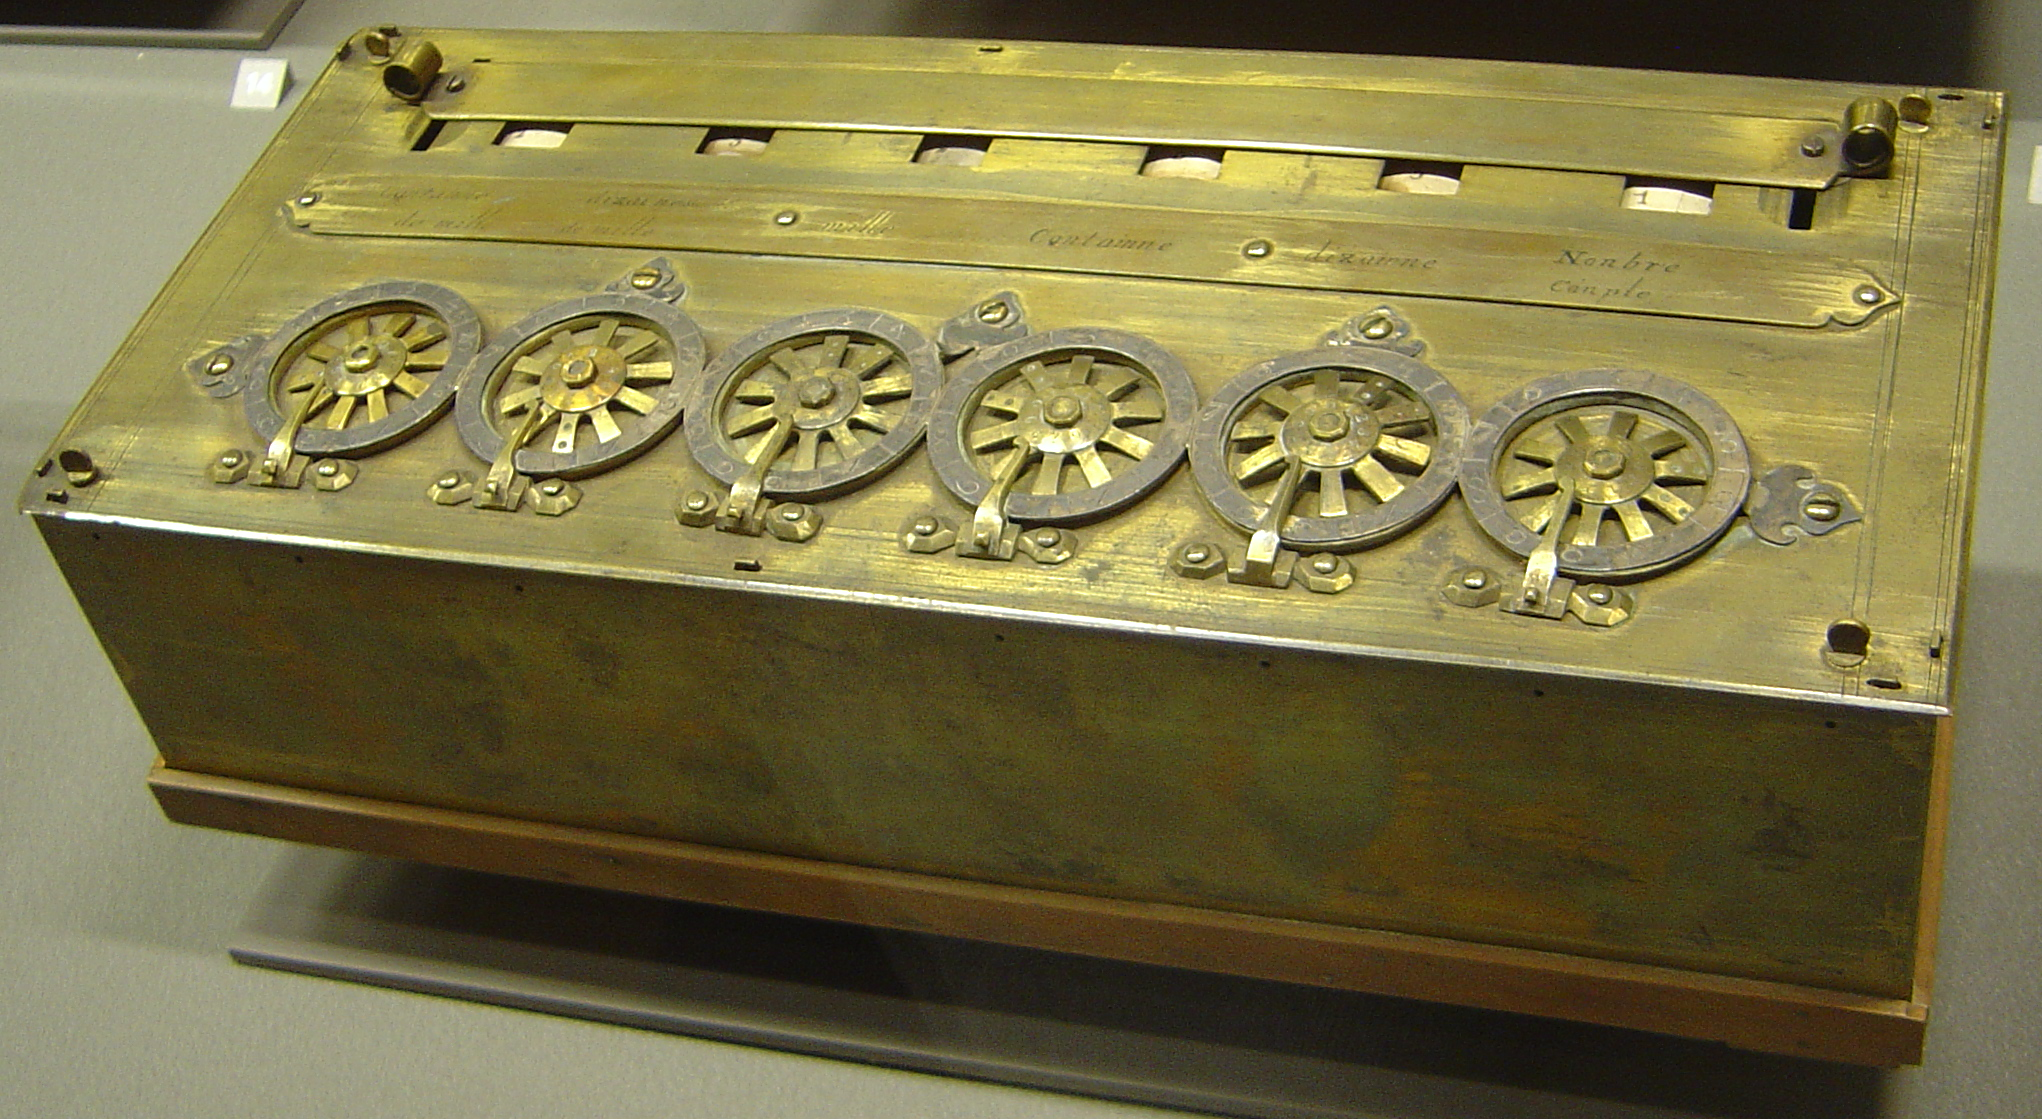
\includegraphics[width=0.9\textwidth]{resources/Pascaline.jpg}
                \caption[]{Paskalina\cite{paskalina}}
            \end{figure}
        \end{columns}
    \end{center}
\end{frame}

\begin{frame}[allowframebreaks]{Dviejų paveikslėlių pavyzdys}
    Du paveikslėlius galima pavaizduoti vienas šalia kito.
    \begin{columns}[b]
        \column{0.5\textwidth}
        \begin{figure}
            \centering
            
\includegraphics[width=0.5\textwidth]{resources/MIF.png}
            \caption{VU MIF logotipas}
            \label{fig:mif-logo1}
        \end{figure}
        \column{0.5\textwidth}
        \begin{figure}
            \centering
            
\includegraphics[width=0.9\textwidth]{resources/VU_logo_lt.png}
            \caption{VU logotipas}
            \label{fig:vu-logo1}
        \end{figure}
    \end{columns}

\break

Taip pat galima pavaizduoti du paveikslėlius vieną šalia kito, padarant, kad jie turėtų bendrą antraštę.

    \begin{figure}
        \subfloat[][VU MIF logotipas]{
        
\includegraphics[width=0.3\textwidth]{resources/MIF.png}
        \label{fig:mif-logo2}
    }
    \subfloat[][VU logotipas]{
        
\includegraphics[width=0.55\textwidth]{resources/VU_logo_lt.png}
        \label{fig:vu-logo2}
    }
    \caption{Bendras abiejų paveiksliukų pavadinimas}
    \label{fig:du-paveiksleliai}
\end{figure}
\end{frame}

\begin{frame}{Algoritmo pavyzdys}
    Čia pateikiamas algoritmo pavyzdys:
    \begin{algorithm}[H]
    \begin{algorithmic}[1]
    \FOR{$i=1$ to $N$}
    \FOR{$j=1$ to $JJJJ$}
    \STATE $energy[i*JJJ+j] =$ 
    $ interpolate(AAA[i*JJJ+j], ZZZ)$
    \ENDFOR
    \ENDFOR
    \end{algorithmic}
    \caption{pseudocode for the calculation of}
    \label{alg:seq}
    \end{algorithm}
\end{frame}

\section{Literatūros šaltiniai}
\begin{frame}[t,allowframebreaks]
    \frametitle{Literatūros šaltiniai}
    \printbibliography
\end{frame}

\end{document}
